\documentclass{article}
%-------------------------------------------------------------------
% Paquetes necesarios
\usepackage[utf8]{inputenc} % Para caracteres especiales
\usepackage[spanish]{babel} % Para idioma español
\usepackage{amsmath, amssymb} % Para matemáticas
\usepackage{geometry} % Para ajustar márgenes 
\usepackage{graphicx} % Para agregar imágenes
\usepackage{float}
\usepackage{listings} % Para mostrar código
\usepackage{xcolor}   % Para colores
\definecolor{codegreen}{rgb}{0,0.6,0}
\definecolor{codegray}{rgb}{0.5,0.5,0.5}
\definecolor{codepurple}{rgb}{0.58,0,0.82}

% Configuración de estilo para Python
\lstdefinestyle{mystyle}{
    backgroundcolor=\color{white},   
    commentstyle=\color{codegreen},
    keywordstyle=\color{magenta},
    numberstyle=\tiny\color{codegray},
    stringstyle=\color{codepurple},
    basicstyle=\ttfamily\small,
    breakatwhitespace=false,         
    breaklines=true,                 
    captionpos=b,                    
    keepspaces=true,                 
    numbers=left,                    
    numbersep=5pt,                  
    showspaces=false,                
    showstringspaces=false,
    showtabs=false,                  
    tabsize=4,
    frame=single % Añade un marco alrededor
}

\lstset{style=mystyle}
%--------------------------------------------------------------------
% Inicio del documento
\begin{document}
%--------------------------------------------------------------------
% Portada
\begin{titlepage}
    
    \noindent % Evita la sangría inicial
    \begin{tabular}{@{}p{0.5\textwidth} p{0.5\textwidth}@{}}
        
\includegraphics[height=3cm, width=0.45\textwidth, keepaspectratio]{logos/uanl.png} & % Imagen izquierda
        \hfill 
\includegraphics[height=3cm, width=0.45\textwidth, keepaspectratio]{logos/fcfm.png} % Imagen derecha
    \end{tabular}
    
    \begin{center}
        \vspace*{2cm} % Espacio vertical
        \textbf{\Large Universidad Autónoma de Nuevo León} \\[2cm]
        
        \textbf{\Large Licenciatura en Ciencias Computacionales} \\[2cm]
        
        \textbf{\Large A10: Regresión Logística en Python} \\[2cm]
    
        \textbf{\large Materia: Inteligencia Artificial} \\[.5cm]
        \textbf{\large Maestro: Luis Ángel Gutiérrez Rodríguez} \\[2cm]
        
        \textbf{\large Rebeca Jaramillo Camarillo} \\[.5cm]
        \textbf{\large Matrícula: 2132988} \\[.5cm]
        \textbf{\large Grupo: 031} \\
        
        \vfill % Espacio vertical para ajustar el contenido al final de la página
        \textbf{\large Fecha: 23 de marzo de 2025} % Fecha automática
    \end{center}
	
\end{titlepage}

%--------------------------------------------------------------------
% Introducción: Explique brevemente qué es la Regresión Logística y su significado.
\section{Introducción}
En estadística, la regresión logística es un tipo de modelo de regresión que sirve para predecir el resultado de una variable categórica. Es decir, la regresión logística se usa para modelar la probabilidad de que una variable categórica tome un determinado valor en función de las variables independientes.
El modelo de regresión logística más habitual es la regresión logística binaria, en la cual solo hay dos posibles resultados: «fracaso» o «éxito» (distribución de Bernoulli). El «fracaso» se representa con el valor 0, mientras que el «éxito» se representa con el valor 1.\\

Por ejemplo, la probabilidad de que un alumno apruebe un examen en función de las horas que ha dedicado al estudio se puede estudiar mediante un modelo de regresión logística. En este caso, suspender sería el resultado de «fracaso» y, por otro lado, aprobar sería el resultado de «éxito».\\

Otros ejemplos:
\begin{itemize}
    \item Clasificar si el correo que llega es Spam o No es Spam.
    \item Dados unos resultados clínicos de un tumor clasificar en “Benigno” o “Maligno”.
    \item El texto de un artículo a analizar es: Entretenimiento, Deportes, Política ó Ciencia.
    \item A partir de historial bancario conceder un crédito o no.
\end{itemize}

\paragraph{}En este documento, se presenta el paso a paso de una actividad de regresión logística en Python, el cual utiliza datos de entrada para clasificar si el usuario que visita un sitio web usa como sistema operativo Windows, Macintosh o Linux. La información de entrada son 4 características de una web que utiliza Google Analytics y son:
\begin{itemize}
    \item Duración de la visita en Segundos
    \item Cantidad de Páginas Vistas durante la Sesión
    \item Cantidad de Acciones del usuario (click, scroll, uso de checkbox, sliders,etc)
    \item Suma del Valor de las acciones (cada acción lleva asociada una valoración de importancia)
\end{itemize}

\paragraph{} Como la salida es discreta, se asignaran los siguientes valores a las etiquetas:
\begin{itemize}
    \item 0 - Windows
    \item 1 - Macintosh
    \item 2 - Linux
\end{itemize}

\newpage
%--------------------------------------------------------------------
% Metodología: Describe los pasos que tomaste para realizar la actividad, incluidos los fragmentos de código.
\section{Metodología}
A continuación, se muestran los pasos para resolver el ejercicio:

\subsection{Importar librerías necesarias} 
\begin{lstlisting}[language=Python]
import pandas as pd
import numpy as np
from sklearn import linear_model
from sklearn import model_selection
from sklearn.metrics import classification_report
from sklearn.metrics import confusion_matrix
from sklearn.metrics import accuracy_score
import matplotlib.pyplot as plt
import seaborn as sb
\end{lstlisting}

\subsection{Leer el archivo csv y cargarlo como un dataset de Pandas}El siguiente código se encarga de cargar y leer los datos de entrada. Además,  permite visualizar información estadística básica del set de datos, así como el numero de registros de cada sistema operativo.
\begin{lstlisting}[language=Python]
dataframe = pd.read_csv(r"usuarios_win_mac_lin.csv")
print(dataframe.head())

print(dataframe.groupby('clase').size())
\end{lstlisting}

\subsection{Visualización de datos} Visualizacio gráfica en fromato de histograma de los cuatro Features de entrada.
\begin{lstlisting}[language=Python]
dataframe.drop('clase', axis=1).hist()
plt.show()

sb.pairplot(dataframe.dropna(), hue='clase', height=4, vars=["duracion", "paginas","acciones","valor"], kind='reg')
plt.show()
\end{lstlisting}

\newpage
\subsection{Crear y entrenar el Modelo de Regresión Logística} Se cargan las variables de las 4 columnas de entrada en X excluyendo la columna “clase” con el métododrop(). En cambio, se agrega la columna“clase” en la variable y. Se ejecuta X.shape para comprobar la dimensión de la matriz con datos de entrada de 170 registros por 4 columnas. Luego se crea el modelo y se ajusta (fit) al conjunto de entradas X y salidas ‘y’.
\begin{lstlisting}[language=Python]
X = dataframe.drop('clase', axis=1)
y = dataframe['clase']
print(X.shape)

model = linear_model.LogisticRegression(max_iter=1000)
model.fit(X,y)
\end{lstlisting}

\paragraph{}Una vez compilado el modelo, se clasifica el conjunto de entradas X utilizando el método “predict(X)” y se revisa que las salidas coincidan con las salidas reales del archivo csv. Luego se confirma cuan bueno fue el modelo utilizando model.score(), el cual devuelve la precisión media de las predicciones.
\begin{lstlisting}[language=Python]
predictions = model.predict(X)
print(predictions)[0:5]
print(model.score(X,y))
\end{lstlisting}

\subsection{Validación del modelo}Se dividen los datos de entrada de
 forma aleatoria (mezclados) utilizando 80\% de registros para entrenamiento y 20\% para validar.
\begin{lstlisting}[language=Python]
validation_size = 0.20
seed = 7
X_train, X_validation, Y_train, Y_validation = model_selection.train_test_split(X, y, test_size=validation_size, random_state=seed)
\end{lstlisting}

\paragraph{}Después, se vuelve a compilar el modelo de Regresión Logística, pero esta vez sólo con 80\% de los datos de entrada.
\begin{lstlisting}[language=Python]
name = "LogisticRegression"
kfold = model_selection.KFold(n_splits=10, shuffle = True, random_state=seed)
cv_results = model_selection.cross_val_score(model, X_train, Y_train, cv=kfold, scoring="accuracy")
msg = "%s: %f (%f)" % (name, cv_results.mean(), cv_results.std())
print(msg)
\end{lstlisting}

\subsection{Reporte de resultados}
\begin{lstlisting}[language=Python]
print("\nMatriz de confusion:")
print(confusion_matrix(Y_validation, predictions))
print("\nReporte de clasificacion:")
print(classification_report(Y_validation, predictions))

# Clasificacion de nuevos valores
X_new = pd.DataFrame({'duracion': [10], 'paginas': [3], 'acciones': [5], 'valor': [9]})
print("\nPrediccion para nuevos datos:", model.predict(X_new))
\end{lstlisting}

\newpage
%--------------------------------------------------------------------
% Resultados: Presenta los resultados de tu análisis de Regresión Logística.
\section{Resultados}
A continuación, se presentan los resultados del análisis de Regresión Lineal Múltiple\\

Primeros 5 valores del dataframe:
\begin{figure}[H]
    \centering
    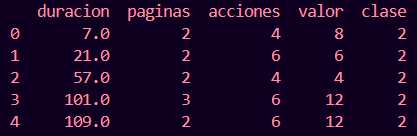
\includegraphics[width=0.6\linewidth]{img/a11_dataframe.png}
    \caption{Paso 2}
    \label{fig:figure2}
\end{figure}

Distribución de clase: 86 usuarios de Windows, 40 usuarios Mac y 44 de Linux 
\begin{figure}[H]
    \centering
    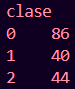
\includegraphics[width=0.1\linewidth]{img/a11_clase.png}
    \caption{Paso 2}
    \label{fig:figure2}
\end{figure}

\newpage
Histogramas de los 4 datos de entrada: “duración”, “páginas”, ”acciones” y “valor” 
\begin{figure}[H]
    \centering
    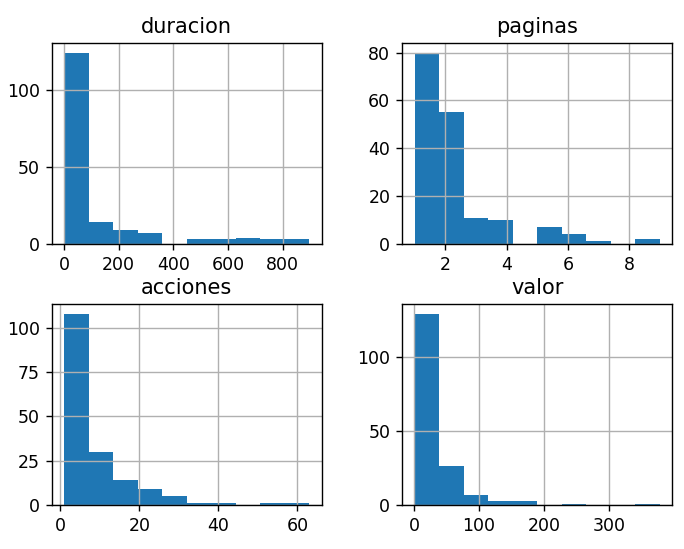
\includegraphics[width=0.8\linewidth]{img/a11_histograma.png}
    \caption{Paso 2}
    \label{fig:figure2}
\end{figure}

\newpage
Interrelación de las entradas de a pares, para ver cómo se concentran linealmente las salidas de usuarios por colores: Sistema Operativo Windows en azul, Mac en en verde y Linux en naranja
\begin{figure}[H]
    \centering
    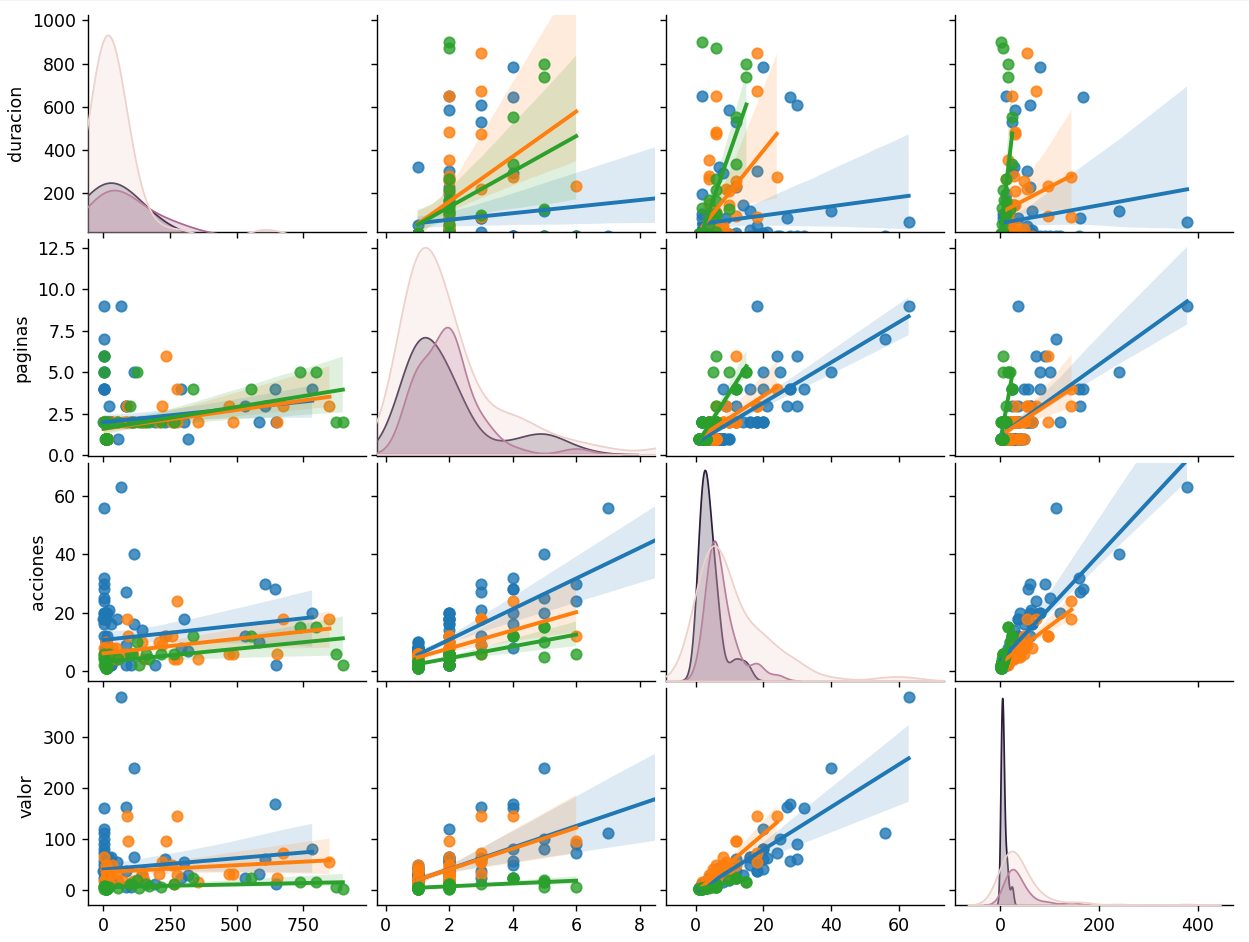
\includegraphics[width=1\linewidth]{img/a11_relacion.png}
    \caption{Paso 2}
    \label{fig:figure2}
\end{figure}

\newpage
La precisión media de las predicciones del modelo es del 77\%.\\
Despues de volver a compilar el modelo de Regresión Logística, pero esta vez sólo con 80\% de los datos de entrada, el nuevo scorig es de 72\%. \\
Luego se hacen las predicciones (clasificación) y el acierto es del 85\%
\begin{figure}[H]
    \centering
    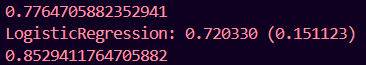
\includegraphics[width=0.5\linewidth]{img/a11_resultados.png}
    \caption{Precisión media de las predicciones}
    \label{fig:figure2}
\end{figure}

Finalmente, se observan los resultados del modelo, como la “matriz de confusión” donde muestra cuantos resultados equivocados tuvo de cada clase (los que no están en la diagonal). En este caso, predijo 3 usuarios que eran Mac como usurarios de Windows, y 2 usuarios Linux que eran Windows.
\begin{figure}[H]
    \centering
    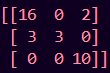
\includegraphics[width=0.2\linewidth]{img/a11_matriz.png}
    \caption{“Matriz de confusión”}
    \label{fig:figure2}
\end{figure}

También se observa el reporte de clasificación con el conjunto de Validación. En este caso, se observa que se utilizaron como “soporte” 18 registros windows, 6 de mac y 10 de Linux (total de 34 registros). Se puede ver la precisión con que se acertaron cada una de las clases, por ejemplo,  de Macintosh tuvo 3 aciertos y 3 fallos (0.5 recall).
\begin{figure}[H]
    \centering
    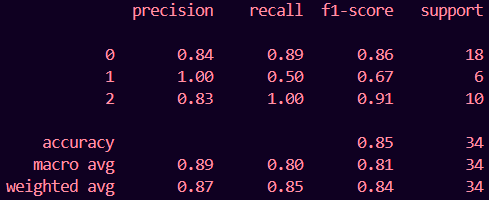
\includegraphics[width=0.8\linewidth]{img/a11_clasificacion.png}
    \caption{Reporte de clasificación}
    \label{fig:figure2}
\end{figure}
\newpage
%--------------------------------------------------------------------
% Conclusión: Resume tus hallazgos y cualquier información obtenida de la actividad.
\section{Conclusión}
Aunque este ejercicio de regresión logística mostró resultados satisfactorios (matriz de confusión, métricas de clasificación y capacidad predictiva para nuevos datos), es importante destacar que se trabajó con un conjunto de datos limitado con fines de aprendizaje. En la práctica, para obtener predicciones más precisas, es necesario utilizar un mayor número de datos (en este caso fueron 170).
%--------------------------------------------------------------------
% Fin del documento
\end{document}